\section{Technology}\label{sec:tech}

  Various technologies will be used to develop OpenDCS, this section is intended
  to provide some common terms and expressions used throughout the document.

  \subsection{ZeroMQ}\label{sec:tech-zmq}

    ZeroMQ is a library that provides a means of creating systems that have
    distributed messaging. From the website (\url{http://zeromq.com}) it offers
    the ability to:

    \begin{itemize}
      \item Connect your code in any language, on any platform.
      \item Carries messages across inproc, IPC, TCP, TIPC, multicast.
      \item Smart patterns like pub-sub, push-pull, and router-dealer.
      \item High-speed asynchronous I/O engines, in a tiny library.
      \item Backed by a large and active open source community.
      \item Supports every modern language and platform.
      \item Build any architecture: centralized, distributed, small, or large.
    \end{itemize}

    Socket types are available to make several patterns possible such as
    Request-Reply (REQ-REP), Publish-Subscribe (PUB-SUB), Parallel Pipelines,
    and Fair Queuing among others. OpenDCS services will initially only be
    developed to use the PUB-SUB and the REQ-REP patterns, but could eventually
    use others. The ability to extend to these others in the future was the
    reason for selecting this library over something else, such as TCP or UDP
    sockets on their own.

    The use of a messaging system to stream data across the different services
    provides an area for innovation. Early research into alternative solutions
    to this project revealed that no other available distributed control system
    that could be found uses a message queueing framework and all rely of
    simple socket types to achieve less performant results than can be seen
    through messaging. Some challenges are expected however, while it is
    straightforward to transmit data over a socket this system will expect the
    messaging equivalents to follow a data exchange format. This will need to
    be created in a fashion that all sides of the communication can implement
    without a great deal of additional effort.

    \paragraph{PUB-SUB Pattern}

      With this form of messaging the publisher sends the message, and the
      subscriber receives them. Messages are meant to be characterized such
      that they be sent without any knowledge of which subscribers will receive
      them, if any at all. Messages can be filtered by the subscriber which
      allows them to receive only the subset that is desired.

      \begin{figure}[H]
        \begin{center}
          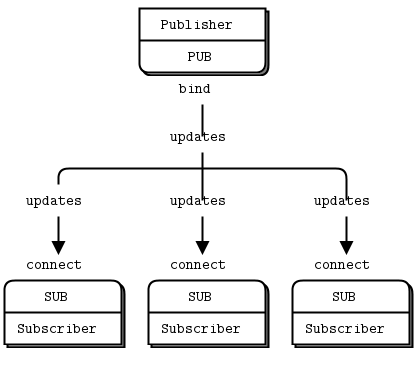
\includegraphics[width=0.5\textwidth]{figures/pub-sub-pattern}
        \end{center}
      \end{figure}

    \paragraph{REQ-REP Pattern}

      This pattern is one of the basic methods that is used in network
      application development to communicate between systems. With this type a
      connection is made and there are a series of transactions until the
      request is complete and a response is provided. A simple example of this
      is browsing a web page, a person using a web browser requests a page and
      the server responds with the page content for the browser to render

      \begin{figure}[H]
        \begin{center}
          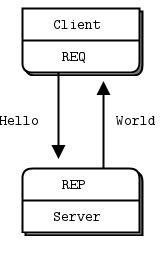
\includegraphics[width=0.25\textwidth]{figures/req-rep-pattern}
        \end{center}
      \end{figure}

  \subsection{Vala}\label{sec:tech-vala}

    Vala is a programming language that aims to bring modern programming
    language features without imposing any runtime requirements and without
    using a different ABI compared to applications and libraries written in
    C~\cite{Vala2016}.

  \subsection{ZLib Compression}\label{sec:tech-zlib}

    One unknown aspect of this project is whether or not the type of data
    created by the system will benefit from compression prior to transmission.
    In order to test this plugins will be devised to compress/decompress data,
    and record measurements of the results. Many compression schemes are
    available, but one that is ubiquitous and available in the libraries being
    used to develop this project is ZLib. ZLib is a compression format that is
    used by all major operating systems to perform backups, reduce log file
    sizes, and in general compress data.

    If successful the use of a compression mechanism in this kind of system
    could be very useful as it makes it possible to send large amounts of data
    as a single compressed package, at a lower cost. This could however result
    in the finding that the data created by the system does not benefit from
    compression, and while this is not known it is suspected. Compression
    algorithms frequently are developed to address a certain type of data, for
    instance JPEG for image data, and it will be a challenge in this project to
    determine if ZLib will be a good fit for the kind of random values that are
    produced by a data acquisition system.
